\documentclass[compress]{beamer}
\usepackage{ifthen,verbatim}

\newcommand{\isnote}{}
\xdefinecolor{lightyellow}{rgb}{1.,1.,0.25}
\xdefinecolor{darkblue}{rgb}{0.1,0.1,0.7}

%% Uncomment this to get annotations
%% \def\notes{\addtocounter{page}{-1}
%%            \renewcommand{\isnote}{*}
%% 	   \beamertemplateshadingbackground{lightyellow}{white}
%%            \begin{frame}
%%            \frametitle{Notes for the previous page (page \insertpagenumber)}
%%            \itemize}
%% \def\endnotes{\enditemize
%% 	      \end{frame}
%%               \beamertemplateshadingbackground{white}{white}
%%               \renewcommand{\isnote}{}}

%% Uncomment this to not get annotations
\def\notes{\comment}
\def\endnotes{\endcomment}

\setbeamertemplate{navigation symbols}{}
\setbeamertemplate{headline}{\mbox{ } \hfill
\begin{minipage}{5.5 cm}
\vspace{-0.75 cm} \small
\end{minipage} \hfill
\begin{minipage}{4.5 cm}
\vspace{-0.75 cm} \small
\begin{flushright}
\ifthenelse{\equal{\insertpagenumber}{1}}{}{Jim Pivarski \hspace{0.2 cm} \insertpagenumber\isnote/\pageref{numpages}}
\end{flushright}
\end{minipage}\mbox{\hspace{0.2 cm}}\includegraphics[height=1 cm]{../cmslogo} \hspace{0.1 cm} \includegraphics[height=1 cm]{../tamulogo} \hspace{0.01 cm} \vspace{-1.05 cm}}

\begin{document}
\begin{frame}
\vfill
\begin{center}
\textcolor{darkblue}{\Large Effect of GlobalPositionRcd-removal Bug \\ \vspace{0.2 cm} on Muon Alignment}

\vfill
\begin{columns}
\column{0.3\linewidth}
\begin{center}
\large
Aysen Tatarinov

Vadim Khotilovich

\textcolor{darkblue}{\it Jim Pivarski}

Alexei Safonov
\end{center}
\end{columns}

\begin{columns}
\column{0.3\linewidth}
\begin{center}
\scriptsize
{\it Texas A\&M University}
\end{center}
\end{columns}

\vfill
 8 June, 2010

\end{center}
\end{frame}

%% \begin{notes}
%% \item This is the annotated version of my talk.
%% \item If you want the version that I am presenting, download the one
%% labeled ``slides'' on Indico (or just ignore these yellow pages).
%% \item The annotated version is provided for extra detail and a written
%% record of comments that I intend to make orally.
%% \item Yellow notes refer to the content on the {\it previous} page.
%% \item All other slides are identical for the two versions.
%% \end{notes}

\small

%% \begin{frame}
%% \frametitle{Outline}
%% \begin{itemize}\setlength{\itemsep}{0.75 cm}
%% \item 
%% \end{itemize}
%% %% \hspace{-0.83 cm} \textcolor{darkblue}{\Large Outline2}
%% \end{frame}

%% \section*{First section}
%% \begin{frame}
%% \begin{center}
%% \Huge \textcolor{blue}{First section}
%% \end{center}
%% \end{frame}

\begin{frame}
\frametitle{Overview (not just this talk)}
\begin{itemize}
\item We confirm the RPC-hit bias presented by Pablo
\begin{itemize}
\item RPC hits were included in track refits because of a typo
\item correcting this fixes sawtooth and residuals vs.\ $q/p_T$ biases
\item $p_T > 100$~GeV/$c$ cut was used to limit the effect on alignment (to 1.5~mm, as it turns out); now this cut can be removed, making alignment with collisions possible
\item \mbox{see \href{http://indico.cern.ch/getFile.py/access?contribId=4&resId=0&materialId=slides&confId=88578}{\tiny http://indico.cern.ch/getFile.py/access?contribId=4\&resId=0\&materialId=slides\&confId=88578}\hspace{-1 cm}}
\end{itemize}
\item Muon POG discovered a strange feature with the new alignment constants
\begin{itemize}
\item low-$p_T$ track seeds assigned a default value of 3.0~GeV/$c$, with a cut to remove them at 3.001~GeV/$c$
\item muon alignment spread this distribution above the cut
\item not an alignment problem, but discovered by muon alignment
\end{itemize}
\item GlobalPositionRcd-removal bug: \textcolor{darkblue}{this talk}
\end{itemize}
\end{frame}

\begin{frame}
\frametitle{GlobalPositionRcd bug-fix}

\begin{itemize}
\item Andreas discovered and corrected an error in the way GlobalPositionRcds are handled in alignment (not track-reco)
\begin{itemize}
\item GlobalPositionRcd must be in geometry to calculate
  residuals
\item it must then be removed from the final results before outputing to TrackerAlignmentRcd/DTAlignmentRcd/CSCAlignmentRcd
\item rotations {\it (only)} were improperly removed
\end{itemize}
\end{itemize}

\vfill
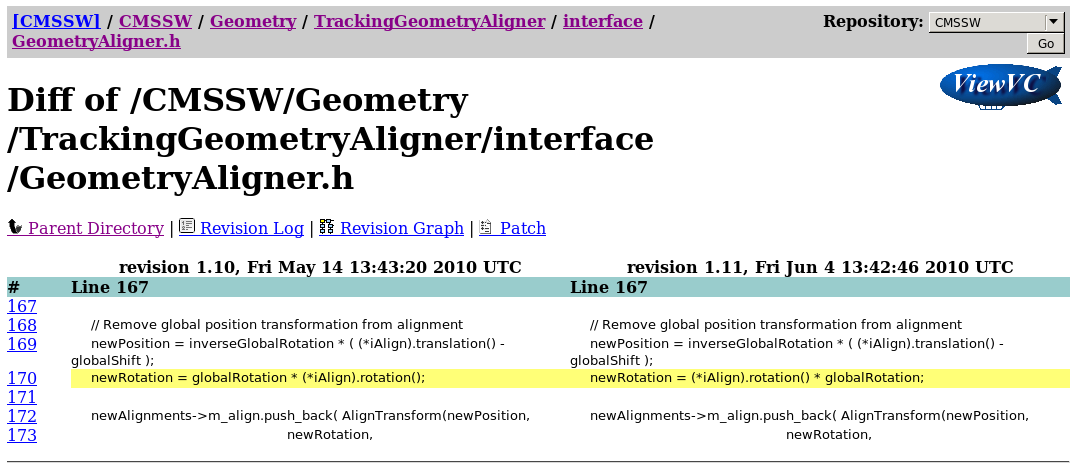
\includegraphics[width=\linewidth]{codeupdate.png}
\end{frame}

\begin{frame}
\frametitle{Effect on DTAlignmentRcd}

\begin{itemize}
\item Plotting: (alignment fit output) $-$ (change in DTAlignmentRcd) for each chamber; can only be non-zero if $\exists$ error in AlignmentProducer
\end{itemize}

\vspace{-0.3 cm}
\begin{center}
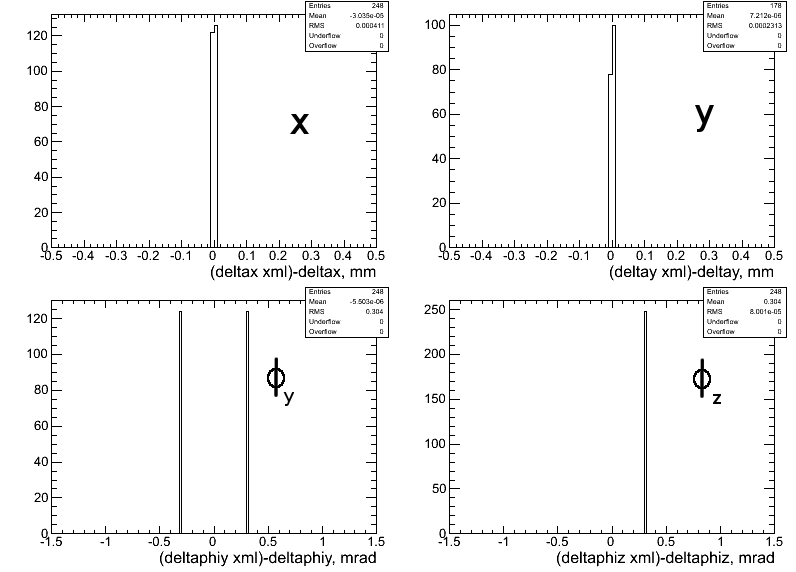
\includegraphics[width=0.75\linewidth]{delta_deltas__g6__05.png}
\end{center}

\vspace{-0.3 cm}
\begin{itemize}
\item After alignment results were sent to AlignmentParameters,
  \mbox{$\pm$0.3~mrad\hspace{-0.5 cm}} \\ artificially added to chamber angles, nothing to chamber
  positions

{\tt gamma} = 0.3~mrad in muon GlobalPositionRcd entry: clear sign
\end{itemize}
\end{frame}

\begin{frame}
\frametitle{Effect on DTAlignmentRcd}
\begin{itemize}
\item After Andreas fixed it, the alignment fit results are almost
  exactly equal to what is found in final DTAlignmentRcd (note smaller scale)
\end{itemize}

\vspace{-0.3 cm}
\begin{center}
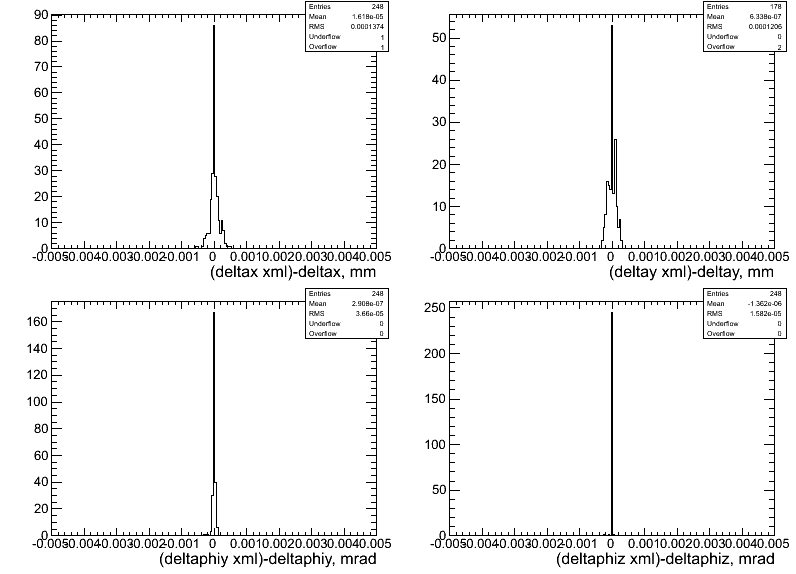
\includegraphics[width=0.65\linewidth]{delta_deltas__g6_with_andreas_bug_fix__05.png}
\end{center}

\vspace{-0.3 cm}
\begin{itemize}
\item This is {\it similar} to things that the Muon Alignment Quality
  Browser already checks; it is being added to the suite of automated tests
\item Also investigating remaining differences: related to
  single-precision floats in DataFormats/GeometrySurface/interface/Surface.h?
\end{itemize}
\end{frame}

\begin{frame}
\frametitle{What was affected and how?}
\begin{itemize}\setlength{\itemsep}{0.2 cm}
\item CRAFT-10 DT alignment
\begin{itemize}
\item $\pm$0.3~mrad in $\phi_y$, $\phi_z$ in first alignment pass (iteration)

\item but effects are nearly cumulative when the procedure is iterated (see next pages)

\item 5 iterations $\to$ at most 1.5~mrad errors
\end{itemize}

\item CRAFT-10 CSC alignment was {\it not} affected
\begin{itemize}
\item beam-halo step (internal) was performed with GlobalPositionRcd = (0,0,0,0,0,0)
\item disk alignment step uses GlobalPositionRcd, but not in AlignmentProducer
\end{itemize}

\item Tracker alignments should be unaffected because tracker
  GlobalPositionRcd entry has no rotation
\end{itemize}
\end{frame}

\begin{frame}
\frametitle{Effect on DT alignment}

\begin{itemize}
\item Plotting (DTAlignmentRcd entries with bug) $-$ (without bug)
\item \only<1>{\textcolor{darkblue}{Iteration 1}} \only<2>{\textcolor{darkblue}{Iteration 2}} \only<3>{\textcolor{darkblue}{Iteration 3}} \only<4>{\textcolor{darkblue}{Iteration 4}} \only<5>{\textcolor{darkblue}{Iteration 5} (last)}
\end{itemize}
\begin{columns}
\column{0.65\linewidth}
\only<1>{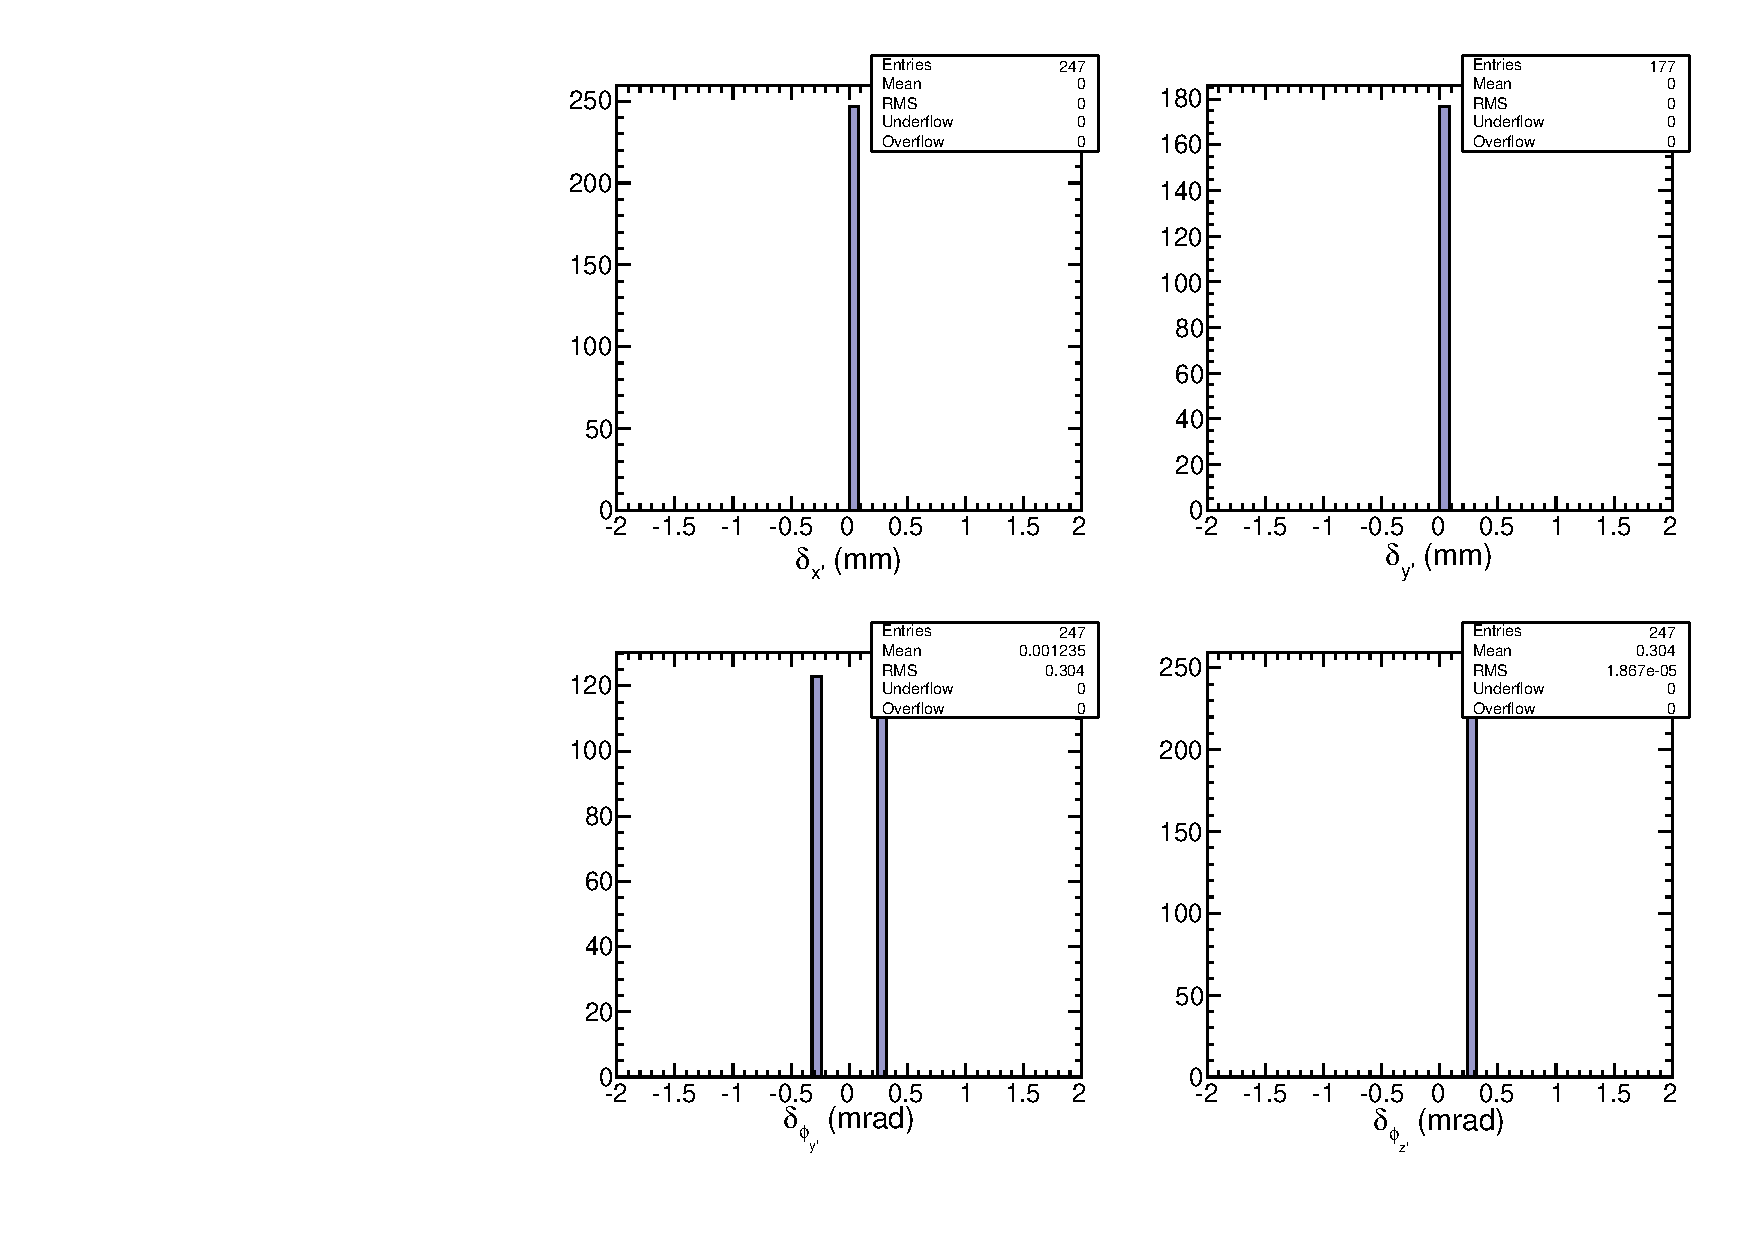
\includegraphics[width=\linewidth]{01_xml_before_and_after_bug_fix_iter1.pdf}}
\only<2>{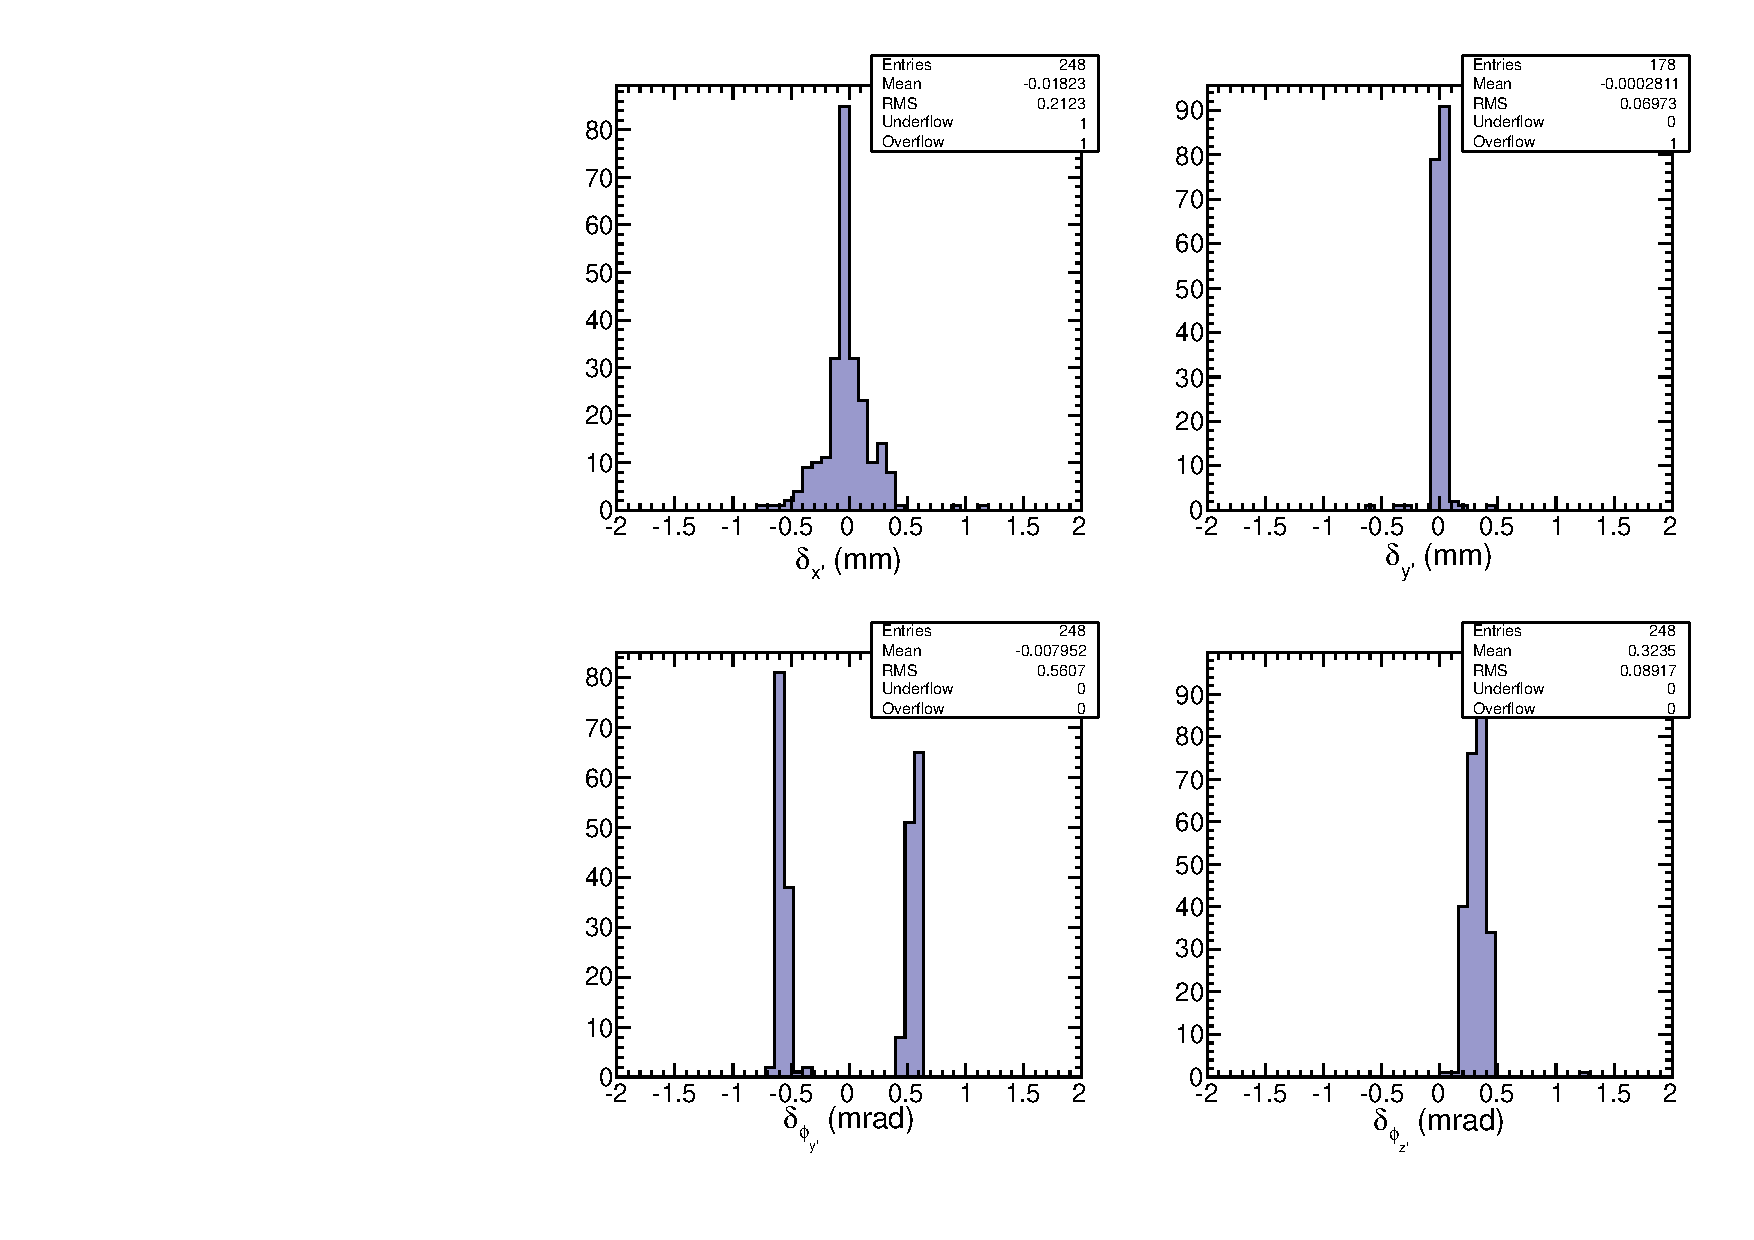
\includegraphics[width=\linewidth]{02_xml_before_and_after_bug_fix_iter2.pdf}}
\only<3>{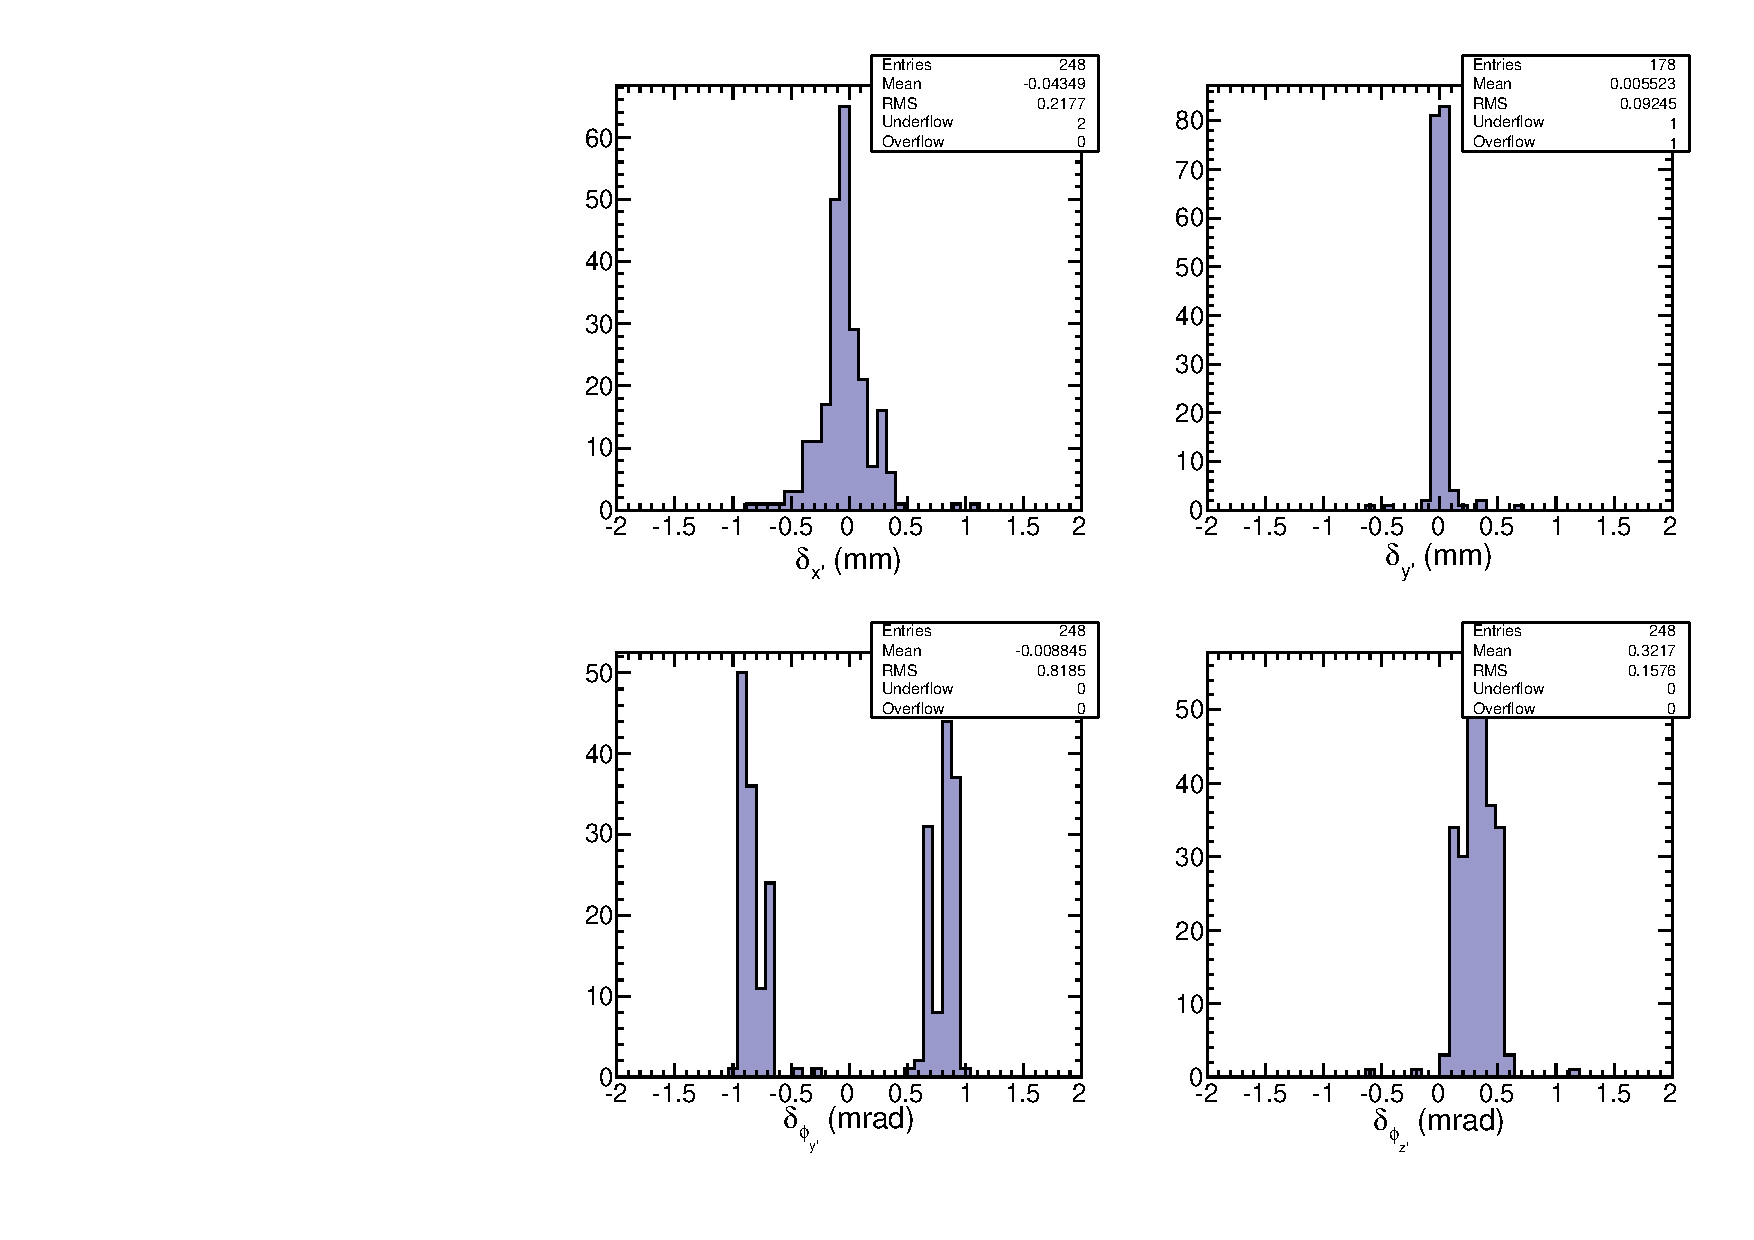
\includegraphics[width=\linewidth]{03_xml_before_and_after_bug_fix_iter3.pdf}}
\only<4>{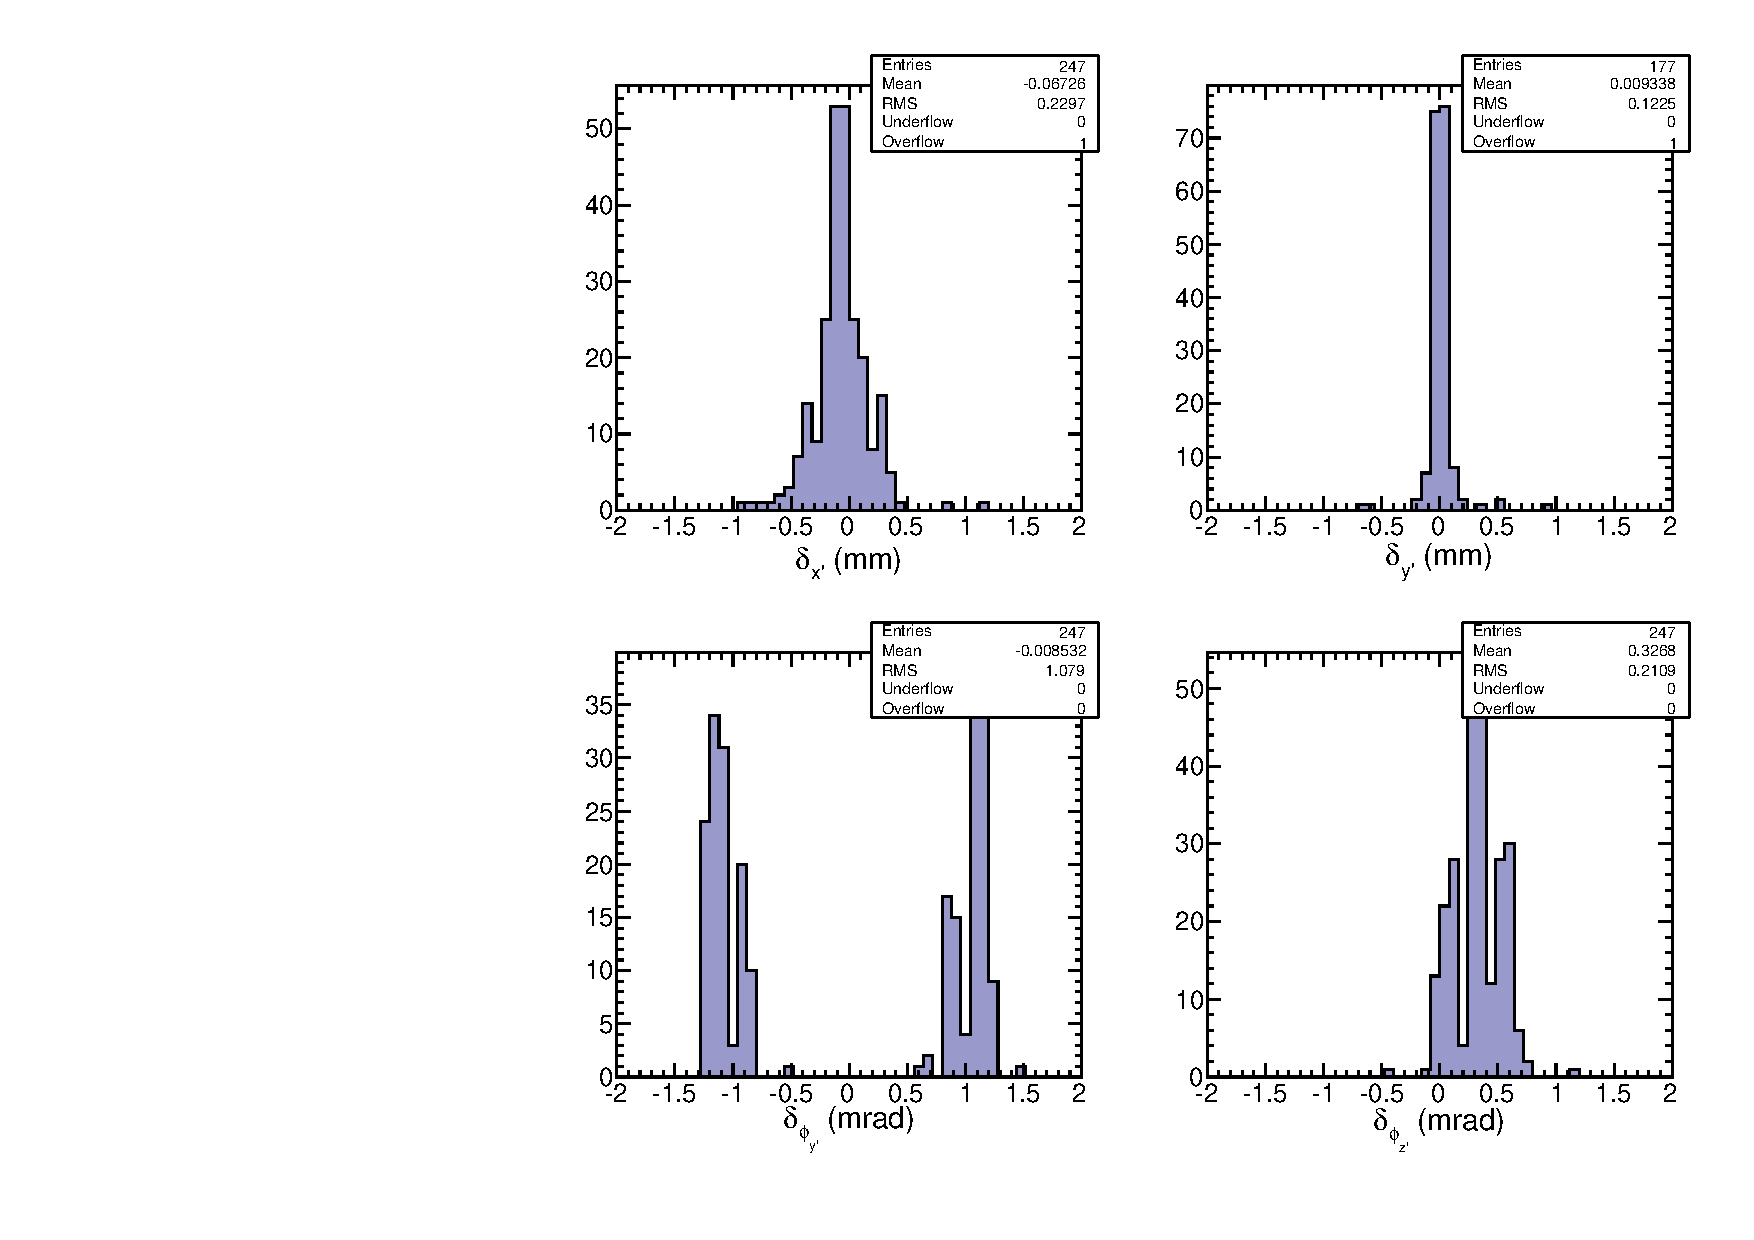
\includegraphics[width=\linewidth]{04_xml_before_and_after_bug_fix_iter4.pdf}}
\only<5>{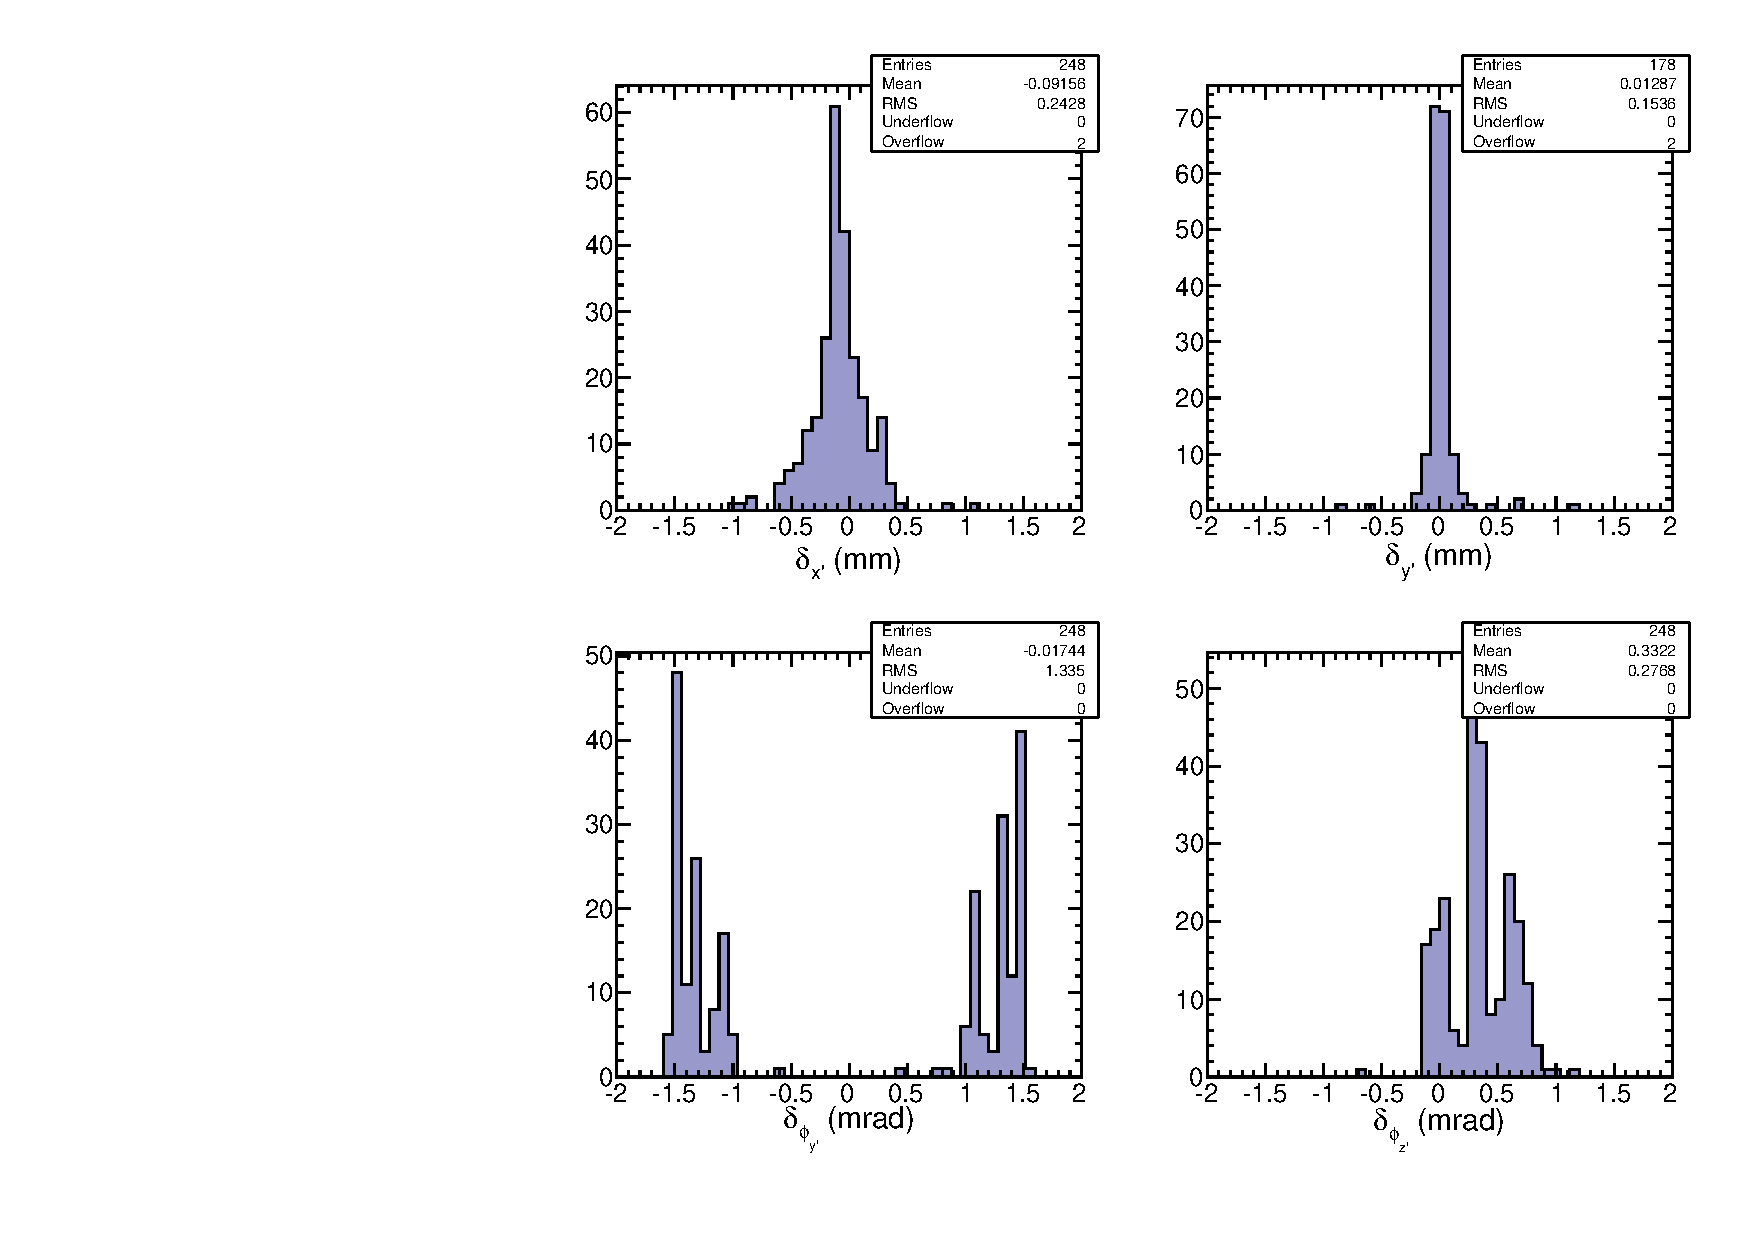
\includegraphics[width=\linewidth]{05_xml_before_and_after_bug_fix_iter5.pdf}}

\column{0.35\linewidth}

\begin{itemize}
\item First iteration differences are exactly $\pm$0.3~mrad
\item Subsequent iterations mix $\phi_y$/$\phi_z$ and $x$ (spread by 250~microns)
\item $\phi_y$ grows linearly, $\phi_z$ is roughly constant
\item Peaks correspond to different wheels
\end{itemize}

\end{columns}
\end{frame}

\begin{frame}
\frametitle{Conclusions}

\begin{itemize}\setlength{\itemsep}{0.25 cm}
\item GlobalPositionRcd-removal is a necessary part of AlignmentProducer

\item It was being performed incorrectly, with $x \sim 0.25$~mm, \\ $\phi_y$, $\phi_z \sim 1.5$~mrad effects on CRAFT-10 DT alignment
\begin{itemize}
\item a different effect from RPC-hit bias
\end{itemize}

\item Unrelated to track-based/hardware ``twist'' discrepancy
\begin{itemize}
\item that was present in raw residuals in the first iteration
\item and is much larger (4~mm between wheels $\pm$2)
\end{itemize}

\item Does not affect CRAFT-10 CSC alignment

\item Similar to tests in Muon Alignment Quality Browser ($\mu$AQB)
\begin{itemize}
\item $\mu$AQB previously only tested $x$ for this kind of divergence
\item adding checks for all alignment parameters
\end{itemize}
\end{itemize}

\label{numpages}
\end{frame}

\end{document}
